% !TEX root = ../entropy.tex

\section{Data}%
\label{sec:data}

\subsection{Preprocessing}%
\label{sub:preprocessing}

Duplicate transactions


\subsection{Sample selection}%
\label{sub:sample_selection}

\begin{table}[ht]
\caption{Sample selection}\label{tab:selection}
\begin{tabular}{lrrrr}
\toprule
                                                 &  Users & Accounts & Transactions & Value (\pounds M) \\
\midrule
                                      Raw sample & 24,163 &  123,625 &   59,647,019 &          11,209.7 \\
                       At least 6 months of data & 21,508 &  117,000 &   59,088,076 &          11,116.8 \\
                               No missing months & 18,550 &   98,513 &   51,252,412 &           9,606.4 \\
                      Account balances available & 14,714 &   85,590 &   44,163,629 &           8,618.7 \\
At least 5 debits totalling \pounds200 per month & 12,296 &   70,981 &   38,618,825 &           7,469.7 \\
                    At least one current account & 12,148 &   70,366 &   38,280,116 &           7,421.9 \\
            Income in 2/3 of all observed months &  9,963 &   60,151 &   33,270,455 &           6,490.2 \\
 Yearly income between \pounds5k and \pounds200k &  6,716 &   36,829 &   21,460,727 &           3,677.9 \\
            No more than 10 accounts in any year &  6,169 &   26,999 &   18,241,355 &           2,855.1 \\
      Debits of less than \pounds100k each month &  5,760 &   24,486 &   16,409,561 &           1,998.7 \\
                                    Final sample &  5,760 &   24,486 &   16,409,561 &           1,998.7 \\
\bottomrule
\end{tabular}

\end{table}


\subsection{Sample description}%
\label{sub:sample_description}

\begin{figure}[h]\center
    \caption{Distribution of user incomes}    
    \label{fig:income_distr}
    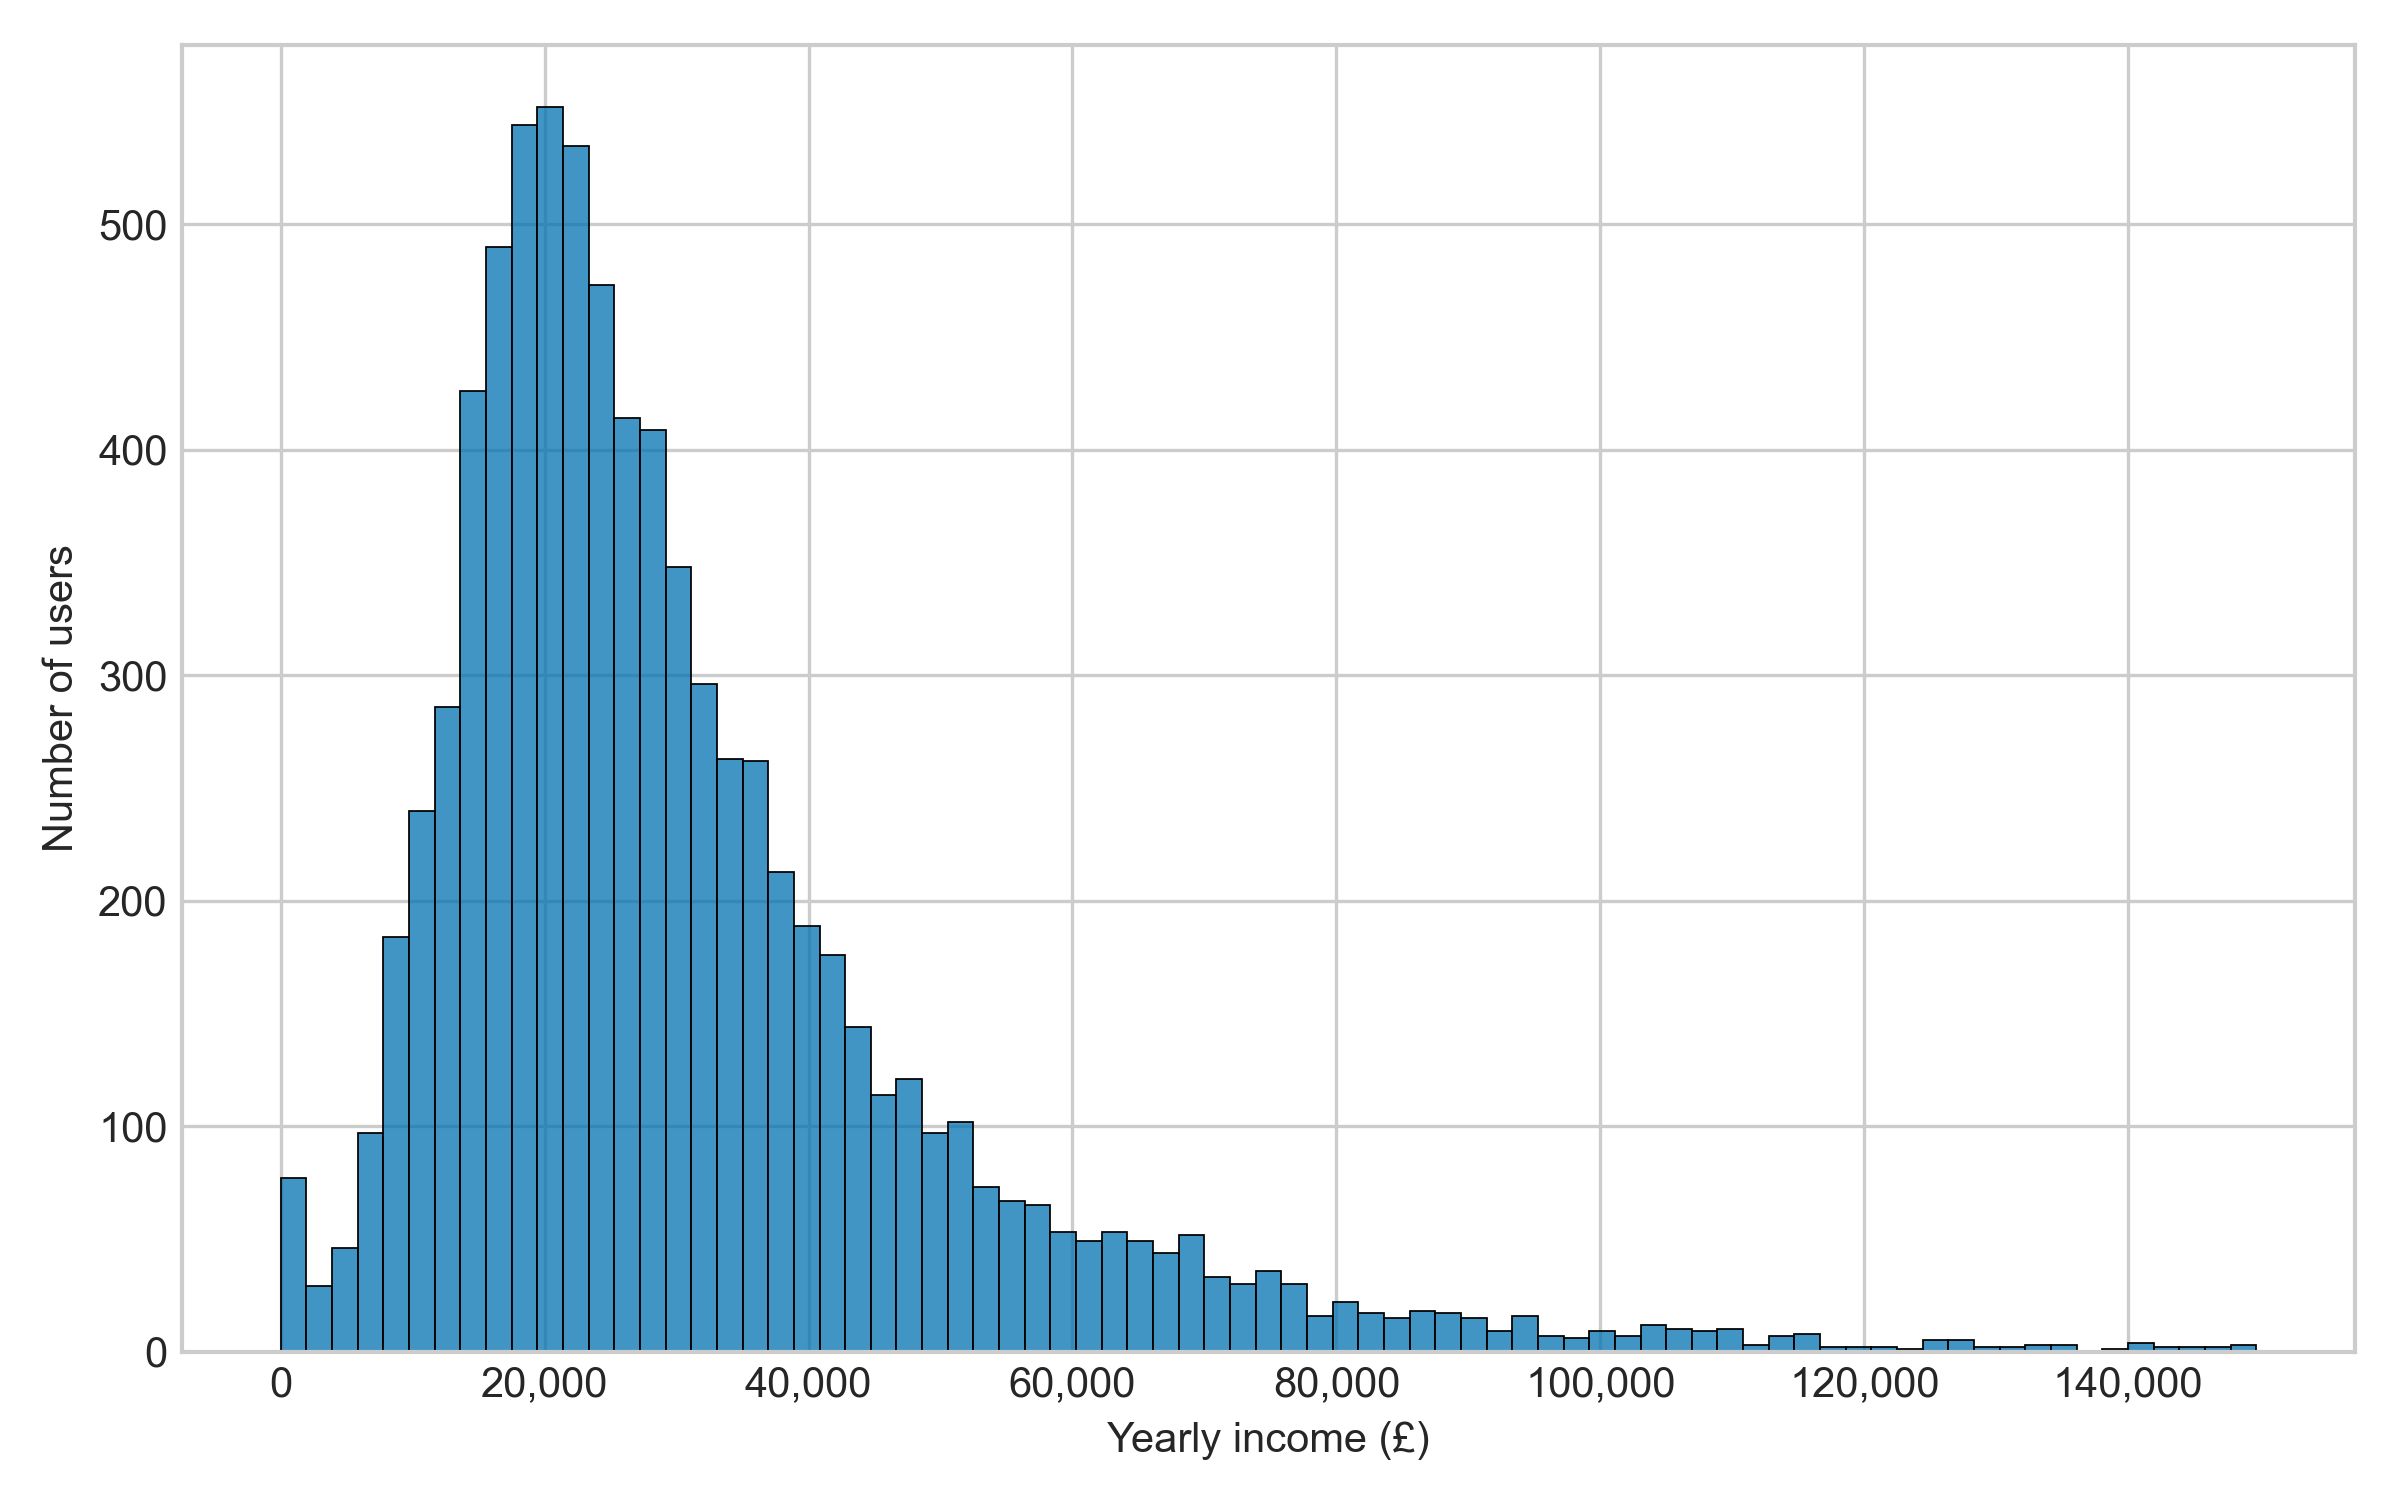
\includegraphics[width=0.9\textwidth]{\figdir/user_income_hist.png}
\end{figure}

\begin{figure}[h]\center \newcommand\width{.9\textwidth} \caption{Monthly
        transactions by account type}    \label{fig:monthly_txns}
        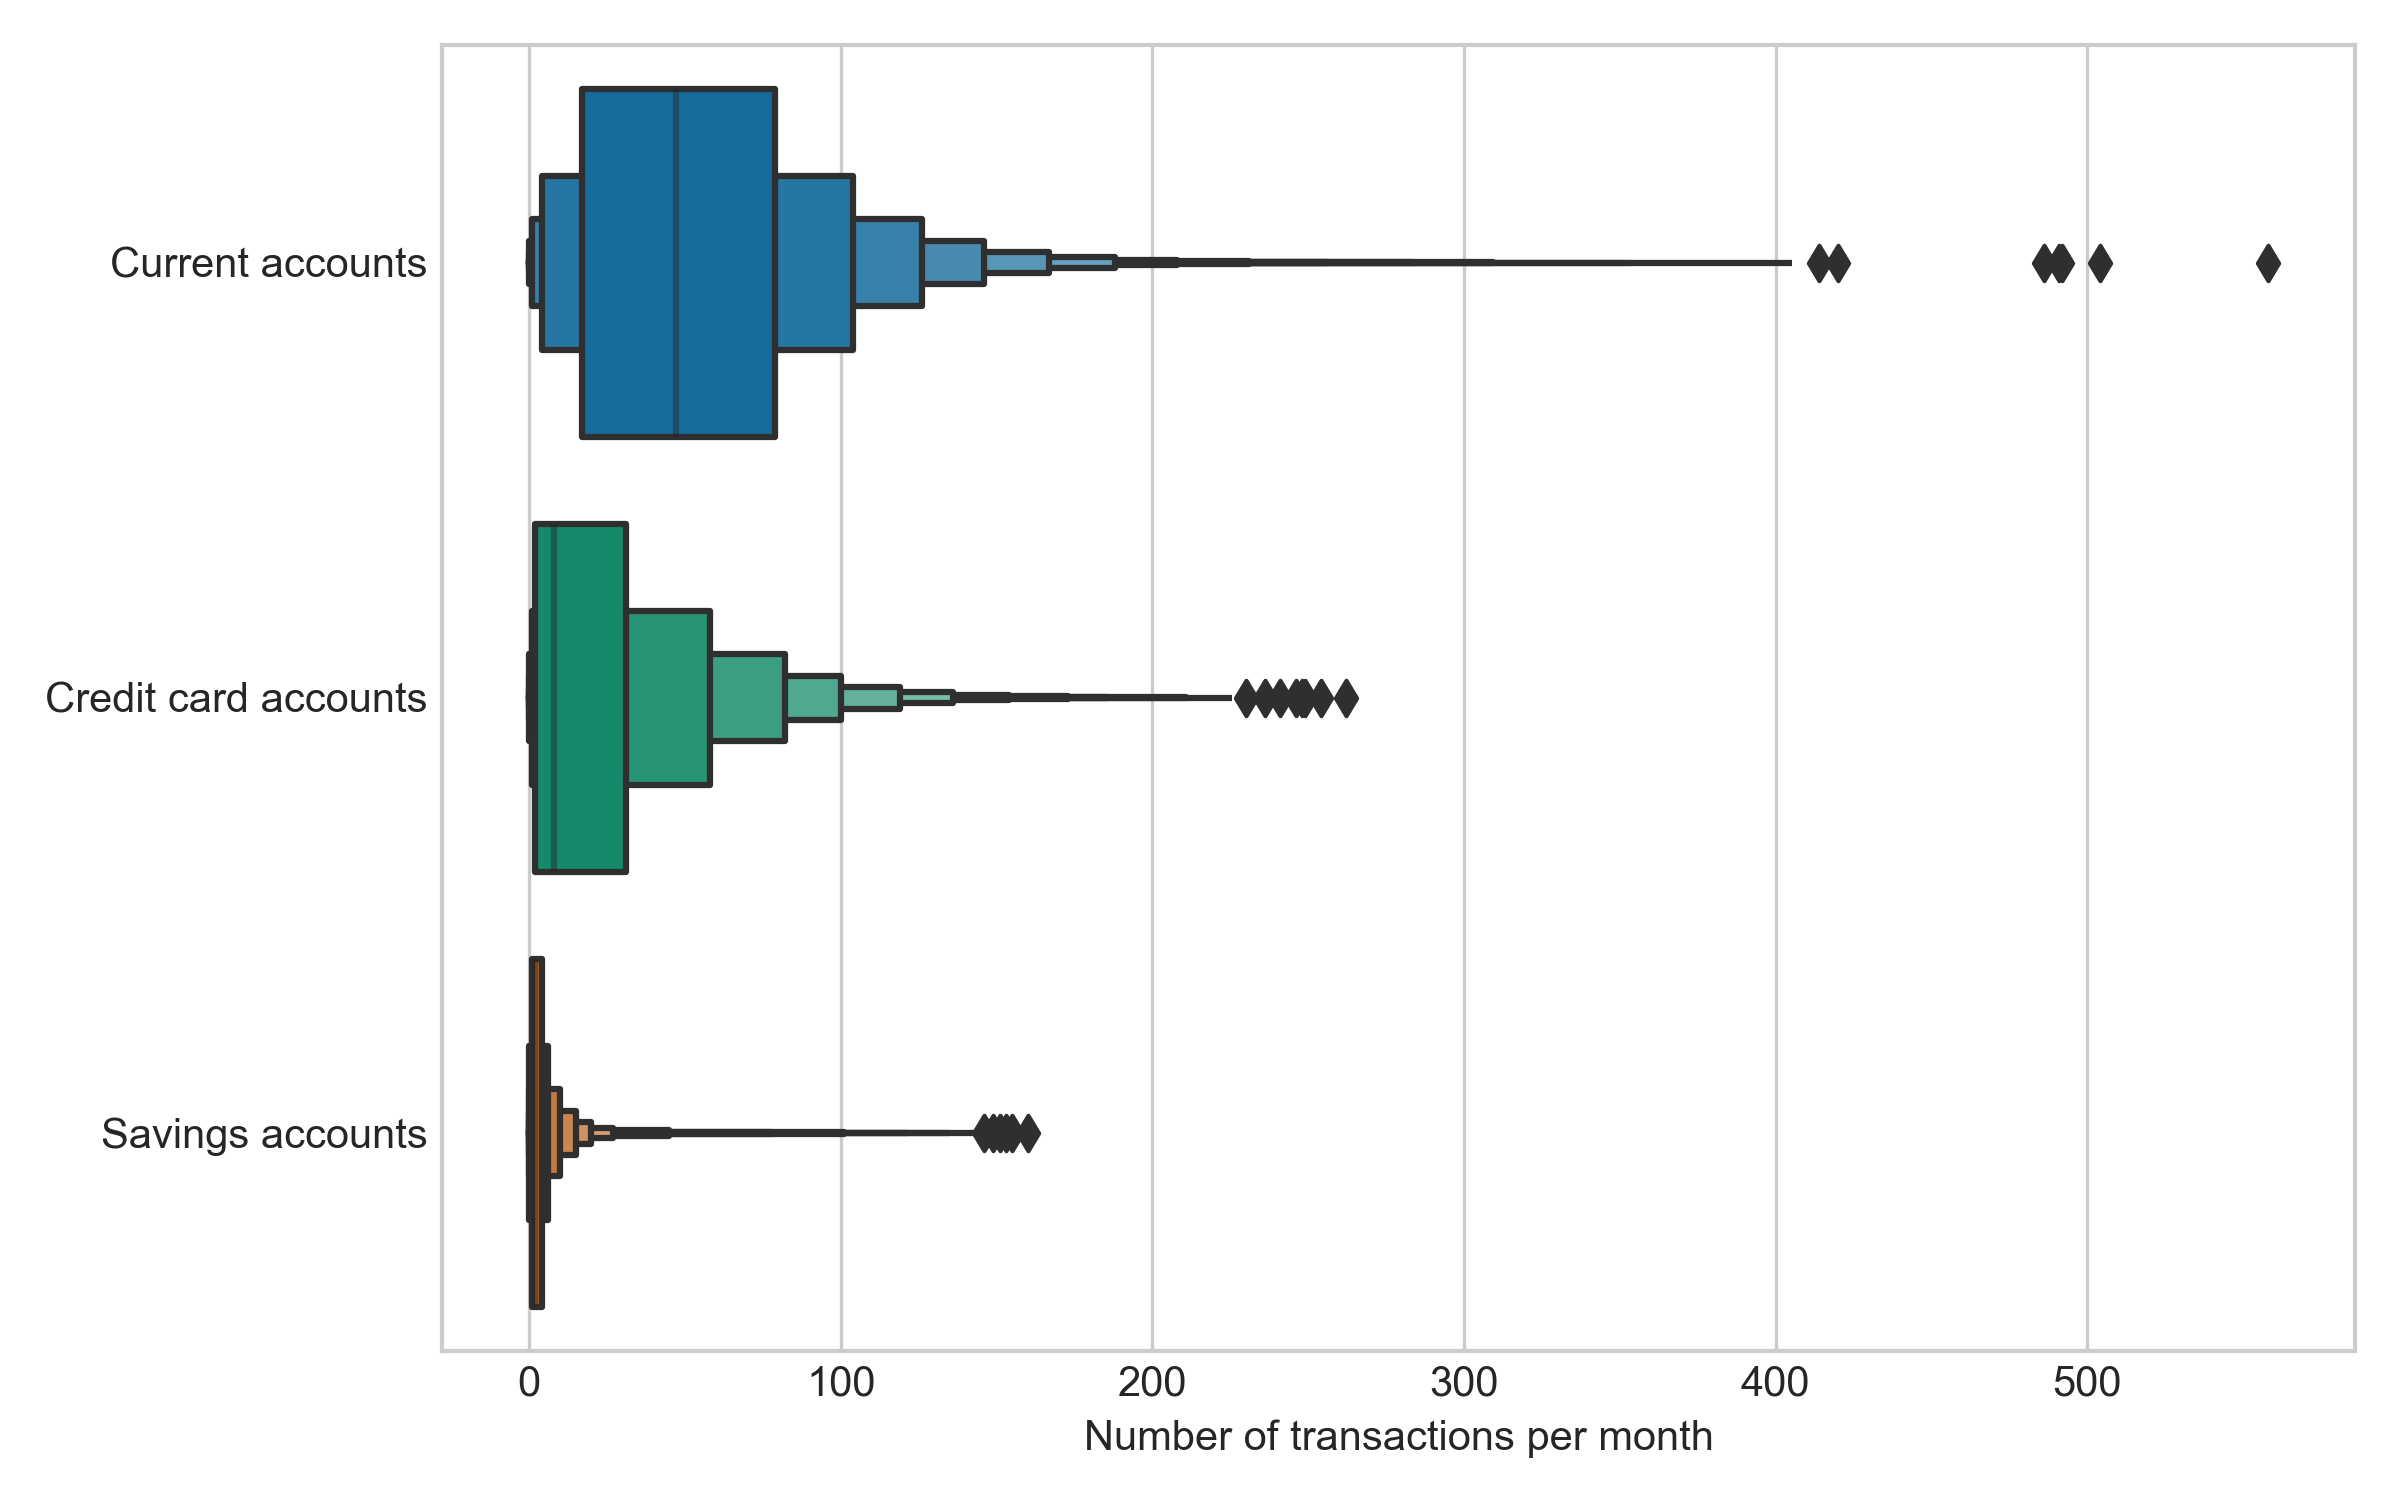
\includegraphics[width=\width]{\figdir/num_txns_by_account_type.png}
        \fignote{\width}{The two innermost boxes in the
            \href{https://vita.had.co.nz/papers/letter-value-plot.html}{letter-value
            plots} are identical to those in a boxplot, with the center line
            corresponding to the median and the left and right edges to the
            first and third quartiles, respectively -- or half of the remaining
            data on either side of the median.  Additional boxes on either side
            extend that principle by corresponding to half of the remaining
            data on that side. For instance, the second box to the right of the
            median in the current accounts plot indicates that half of all
            account-month observations to the right of the third quartile have
            fewer than about 105 transactions. Boxes of the same height
            correspond to the same level, individually drawn observations are
        outliers.}
\end{figure}



\subsection{Dependent variable}%
\label{sub:dependent_variable}

Types of balances, from \citet{becker2017does}, who treats balance at end of
each month as observations:

\begin{itemize}
    \item Current account balance
    \item Debit balance (savings and current account balance)
    \item Pure savings (savings account balance only)
    \item Credit balance (loans and negative current account)
    \item Pure credit (loans only)
    \item Wealth held (debit - credit balance)
\end{itemize}


\subsection{Independent variable}%
\label{sub:independent_variable}


Spending entropy:
\begin{itemize}
    \item We calculate spending entropy using the Shannon entropy
        \textit{H}\citep{shannon1948mathematical}, defined as
        \begin{equation}
            H = -\sum{p_i}log_2(p_i),
        \end{equation}
        where $p_i$ is the probability that an
        individual makes a purchase in spending category $i$. The measure can
        broadly be interpreted as the degree to which an individual's spending
        pattern is predictable, whith a higher score indicating less
        predictability.

    \item To calculate individual entropy scores, we group spending into 9
        spending categories (SC), based on the classification used
        by Lloyds Banking Group as discussed in \citet{muggleton2020evidence}.

    \item Also following that paper, when calculating $p_i$ we use additive
        smoothing and add one to the numerator and $N_{SC}$ to the denominator
        to avoid taking logs of zero counts in cases where an individual makes
        no purchases in a given spending category. $p_i$ is thus calculated as
        \begin{equation}
            p_i = \frac{\text{Count of purchases in $SC_i$} + 1}{\text{Count of
            all purchases} + 9}
        \end{equation}

    \item The right-hand panel in Figure~\ref{fig:entropy_dist} shows the
        distribution of the resulting entropy scores.
\end{itemize}

\begin{figure}[h]\center
    \newcommand\width{\textwidth}
    \caption{Transactions distributions}    
    \label{fig:entropy_dist}
    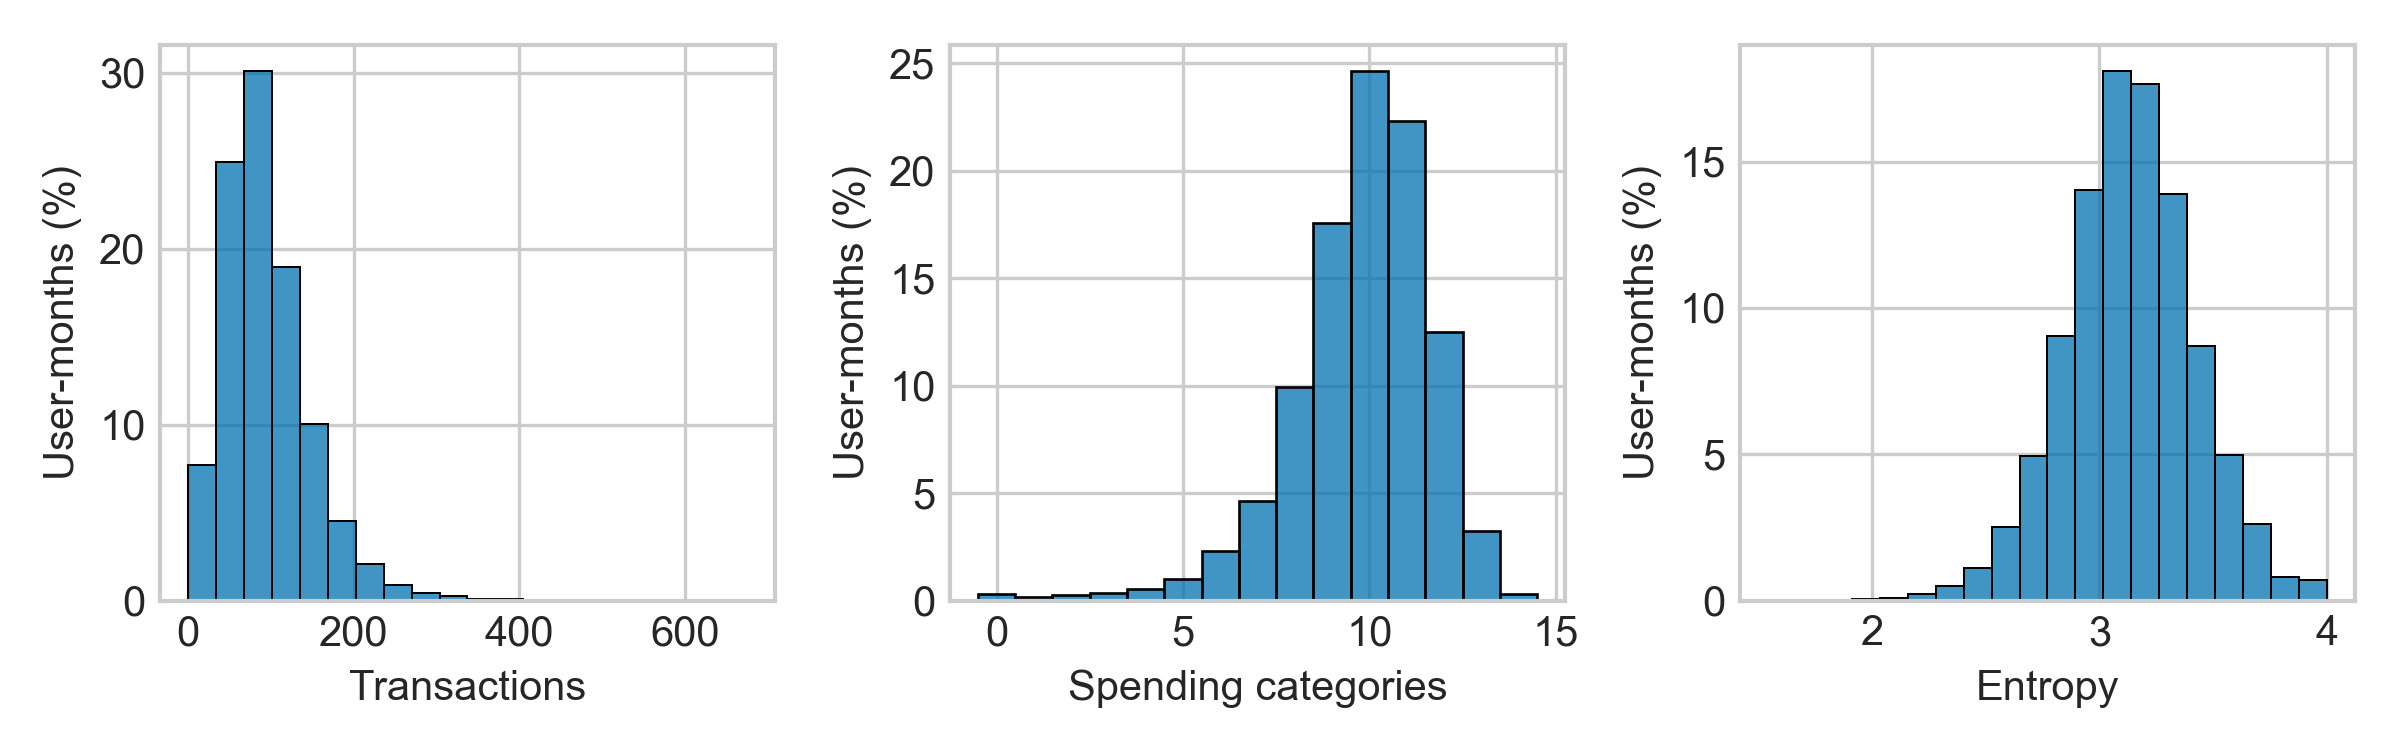
\includegraphics[width=\width]{\figdir/txns_categories_entropy_hists.png}
    \fignote{\width}{Distribution of the number of transactions per user-month
    (left), the number of different spending categories these transactions fall into (middle), and
user-level entropy scores based on these same spending categories (right).}
\end{figure}



